We know that,
\begin{align}
\int_{-\infty}^{\infty}{f_x(x)}\,dx &= 1\\
    \int_{-\infty}^{0}{f_x(x)}\,dx +\int_{0}^{\frac{1}{2}}{f_x(x)}\,dx&\nonumber\\ +\int_{\frac{1}{2}}^{1}{f_x(x)}\,dx +\int_{1}^{\infty}{f_x(x)}\,dx&=1\\
    \int_{0}^{\frac{1}{2}}x\,dx+\int_{\frac{1}{2}}^{1}c(2x-1)^2\,dx&=1\\
    \sbrak{\dfrac{x^2}{2}}_0^\frac{1}{2}+c \sbrak{\dfrac{(2x-1)^3}{6}}_\frac{1}{2}^1&=1\\
    \dfrac{1}{8}+\dfrac{c}{6}&=1\\
    c&=\dfrac{21}{4}
\end{align}
\hspace{2cm}$\therefore$ Required value of $c=\dfrac{21}{4}$

\begin{figure}[h]
   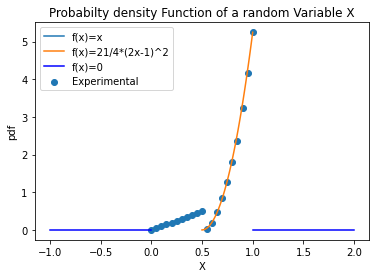
\includegraphics[width=\linewidth]{solutions/ma/2016/10/figures/plot.png}
    \caption{Experimental and Theoritical pdf of X}
    \label{fig:my_label}
\end{figure}



